%\documentclass[dvipdfmx]{beamer}      % platex の場合
\documentclass{beamer}                 % lualatex の場合
\usepackage{mySld}
\usepackage{multicol}

\begin{document}
\title{基礎コンピュータ工学\\第5章 機械語プログラミング\\(パート12)}
\date{}

\begin{frame}
  \titlepage
\end{frame}

%==============================================================================
%\begin{frame}
%  \frametitle
%  \tableofcontents
%\end{frame}

\section{入出力}
%==============================================================================
\begin{frame}
  \frametitle{TeCの構成を思い出してみる}
  \centerline{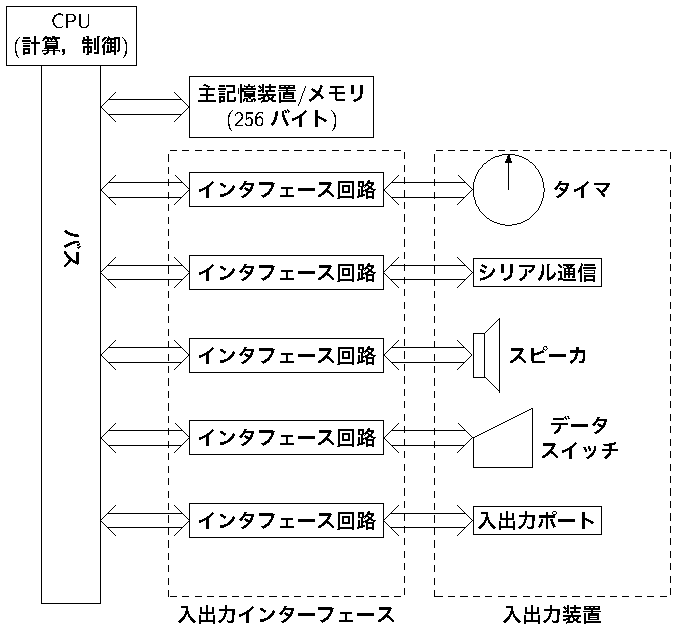
\includegraphics[scale=0.67]{../Tikz/kousei2.pdf}}
  入出力装置を操作するにはどうしたら良いのか?
\end{frame}

%==============================================================================
\begin{frame}
  \frametitle{メモリ領域とI/O領域}
  メモリ領域とは別に,\\
  入出力インタフェースを配置したI/O領域がある.
  \vfill
  \begin{minipage}{0.48\columnwidth}
  \centerline{\footnotesize\begin{tabular}{| c | l |}
    \multicolumn{2}{c}{メモリ領域} \\
    \hline
    番地 & \multicolumn{1}{|c|}{内容} \\
    \hline
    00  &          \\
    01  &          \\
    ... & \multicolumn{1}{|c|}{RAM} \\
    ... & \multicolumn{1}{|c|}{自由に使用可能} \\
    DA  &          \\
    DB  &          \\
    \hline
    DC  &          \\
    ... & \multicolumn{1}{|c|}{システム領域} \\
    FF  &          \\
    \hline
    \end{tabular}
  }
  \begin{center}
  LD,ST,ADD...命令で使用\\
  (プログラムもここに置いた)
  \end{center}
  \end{minipage}
  \begin{minipage}{0.48\columnwidth}
  \centerline{\footnotesize\begin{tabular}{| c | l |}
    \multicolumn{2}{c}{I/O領域} \\
    \hline
    番地 & \multicolumn{1}{|c|}{内容} \\
    \hline
    0   &  Data-Sw/b0:Beep     \\
    1   &  Data-Sw/b0:Spk      \\
    2   &  SIO-Data            \\
    3   &  SIO-Clt/Stat        \\
    ... &  ...                 \\
    F   &  空き/空き           \\
    \hline
    \end{tabular}
  }
  \begin{center}
  IN,OUT命令で使用
  \end{center}
  \end{minipage}
  \vfill
  \vfill
\end{frame}

%==============================================================================
\begin{frame}
  \frametitle{I/Oマップ(I/O領域内の配置を書いたもの)}
  I/O領域の内容を表す\emph{I/Oマップ}がある.
  \vfill
  %\centerline{
    \footnotesize\begin{tabular}{| c | l | l |}
    \hline
    \multicolumn{3}{|c|}{I/Oマップ} \\
    \hline
    番地 & \multicolumn{1}{|c|}{Read} & \multicolumn{1}{|c|}{Write} \\
    \hline
    0 & データスイッチ   & ブザー \\
    1 & データスイッチ   & スピーカ \\
    2 & SIO受信データ    & SIO送信データ \\
    3 & SIOステータス    & SIOコントロール \\
    4 & タイマ現在値     & タイマ周期 \\
    5 & タイマステータス & タイマコントロール \\
    6 & 空き             & INT3コントロール \\
    7 & PIO入力ポート    & PIO出力ポート \\
    8 & ADC CH0          & 空き \\
    9 & ADC CH1          & 空き \\
    A & ADC CH2          & 空き \\
    B & ADC CH3          & 空き \\
    C & 空き             & PIOコントロール \\
    D & 空き             & 空き \\
    E & 空き             & 空き \\
    F & 空き             & 空き \\
    \hline
    \end{tabular}
  %}
  \vfill
  \vfill
\end{frame}

%==============================================================================
\begin{frame}
  \frametitle{IN(Input)命令(入力命令)}
  I/O領域からデータを\emph{入力(Read)}し結果をレジスタに格納する.
  \vfill
  \begin{description}
  \item[フラグ:] 変化しない.
    \vfill
  \item[ニーモニック:]\texttt{IN GR,P}~~~~~~~~~\texttt{(GR ← IO[P])}
    \vfill
  \item[命令フォーマット:] 2バイトの長さを持つ.\\
    {\small\twoByte{$1100_2$}{\GR~$00_2$}{\PP}}
    \vfill
  \item[フローチャート:] 平行四辺形の中に説明を書く.\\
    \centerline{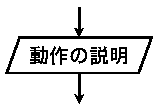
\includegraphics[scale=0.8]{../Tikz/in.pdf}}
    \vfill
  \end{description}
  \vfill
\end{frame}

%==============================================================================
\begin{frame}
  \frametitle{IN(Input)命令の使用例}
  データスイッチの値をデータランプに表示する.
  \vfill
  {\ttfamily\footnotesize
    \begin{tabular}{|l| l l |l|l l|}
      \hline
      番地 & \multicolumn{2}{|c|}{機械語} & 
      ラベル & \multicolumn{2}{|c|}{ニーモニック} \\
      \hline
      00 & C0 & 00 & START & IN   & G0,0    \\
      02 & A0 & 00 &       & JMP  & START   \\
      \hline
    \end{tabular}
  }
  \vfill
  \begin{itemize}
  \item 無限ループになっているので停止しない.
  \item IN命令はI/Oの0番地(データスイッチ)を読む.
  \item IN命令は即座に次の命令に進む(入力待はしない).
  \item プログラムは全速力でループをまわる.
  \item G0を表示した状態でプログラムを実行すると,\\
    データスイッチの値がデータランプに表示され続ける.
  \end{itemize}
  \vfill
\end{frame}

%==============================================================================
\begin{frame}
  \frametitle{IN(Input)命令の応用}
  入力したデータの合計をG0に求める.
  \vfill
  \begin{minipage}{0.43\columnwidth}
    {\ttfamily\small\begin{center}
      \begin{tabular}{|l|l l|}
        \hline
        ラベル & \multicolumn{2}{|c|}{ニーモニック} \\
        \hline
        START & LD   & G0,\#0        \\
        LOOP  & IN   & G1,00H        \\
              & ST   & G1,TMP        \\
              & ADD  & G0,TMP        \\
              & HALT &               \\
              & JMP  & LOOP          \\
        \hline
      \end{tabular}
    \end{center}}
  \end{minipage}
  \begin{minipage}{0.53\columnwidth}
    \begin{enumerate}
    \item[1.] プログラムを入力
    \item[2.] PCに実行開始番地をセット \\
      (0番地ならRESETでも良い)
    \item[3.] G0を表示した状態にする
    \item[4.] データスイッチにデータをセット
    \item[5.] RUNボタンを押す
    \item[6.] データ分,4,5を繰り返す
    \item[7.] データランプに合計表示中
    \end{enumerate}
  \end{minipage}
  \vfill
\end{frame}

%==============================================================================
\begin{frame}
  \frametitle{OUT(Output)命令(出力命令)}
  I/O領域へレジスタのデータを\emph{出力(Write)}する.
  \vfill
  \begin{description}
  \item[フラグ:] 変化しない.
    \vfill
  \item[ニーモニック:]\texttt{OUT GR,P}~~~~~~~~~\texttt{(IO[P] ← GR)}
    \vfill
  \item[命令フォーマット:] 2バイトの長さを持つ.\\
    {\small\twoByte{$1100_2$}{\GR~$11_2$}{\PP}}
    \vfill
  \item[フローチャート:] 平行四辺形の中に説明を書く(INと同じ).\\
    \centerline{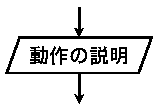
\includegraphics[scale=0.8]{../Tikz/in.pdf}}
    \vfill
  \end{description}
  \vfill
\end{frame}

%==============================================================================
\begin{frame}
  \frametitle{OUT(Output)命令の応用}
  データスイッチ(D0)の操作でブザーを鳴らしたり止めたりする.
  \vfill
  \begin{itemize}
  \item TeCのブザーの仕組み \\
    \vfill
    \centerline{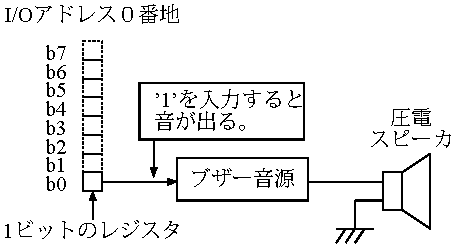
\includegraphics[scale=0.75]{../chap5/buz1.pdf}}
    \vfill
  \item ブザーを鳴らすプログラム \\
    \vfill
    {\ttfamily\footnotesize
      \begin{tabular}{|l| l l |l|l l|}
        \hline
        番地 & \multicolumn{2}{|c|}{機械語} & 
        ラベル & \multicolumn{2}{|c|}{ニーモニック} \\
        \hline
        00 & C0 & 00 & START & IN   & G0,0    \\
        02 & C3 & 00 &       & OUT  & G0,0   \\
        04 & A0 & 00 &       & JMP  & START   \\
        \hline
      \end{tabular}
    }
  \end{itemize}
  \vfill
  ブザーが鳴り続けて困ったらRESETを押す.
  \vfill
\end{frame}

%==============================================================================
\begin{frame}
  \frametitle{まとめ}
  \emph{学んだこと}
  \begin{itemize}
  \item 「\emph{入出力命令}」 = 「IN命令とOUT命令」
  \item \emph{I/O領域とI/Oマップ}
  \item IN命令と応用 \\
    データスイッチの値をデータランプに表示する.\\
    データスイッチから入力した値の合計を求める.\\
  \item OUT命令と応用 \\
    ブザーを鳴らす.\\
  \end{itemize}
  \vfill
  \emph{演習}
  \begin{itemize}
  \item 0で終わるデータ列を入力し合計をX番地に求める.
  \item データスイッチのビット7(D7)でブザーを制御する.
  \end{itemize}
  \vfill
\end{frame}

\end{document}
